\section{Disaggregated Datacenters}
\label{sec:summary}
As briefly outlined in \S\ref{sec:intro}, the scale at which resource disaggregation will happen is, at best, unclear. The goal of this paper is not to advocate any particular architecture for disaggregation datacenters. Nevertheless, we believe that some of the architectural aspects of disaggregated datacenters are inevitable for reasons of feasibility, performance and scalability. 

We start this section by elaborating on our interpretation of a disaggregated datacenter, along with a discussion of some necessary architectural design decisions and the rationale behind these decisions (\S\ref{ssec:arch}). We then make some important assumptions regarding the usage model, implementation and execution of computing frameworks on this architecture (\S\ref{ssec:assumptions}) that allow us to explore the three questions outlined in \S\ref{sec:intro}. Finally, in \S\ref{ssec:summary}, we give a high-level overview of the experimental and simulation setup used in our study.

\subsection{Resource Disaggregation}
\label{ssec:arch}
The high-level idea behind a disaggregated datacenter is illustrated in Figure~\ref{fig:disaggregated}. Each resource type --- CPU, memory, storage, network interfaces as well as specialized components (GPUs, various ASIC accelerators, etc.) --- is developed as a standalone hardware ``blade''. Depending on the scale of disaggregation, individual blades or a collection thereof form the edge of the network, with a direct interface to the network fabric. We discuss below the design and implementation of these individual blades, guided by the feasibility and limitation of the fabric that interconnects these blades. Table~\ref{tab:tech} shows the typical latency and bandwidth for the interconnects within a server-centric architecture. 

\paragraphb{CPU blades}
Given the strict latency and bandwidth requirements of CPU-to-CPU and CPU-to-memory, it seems unlikely that the corresponding traffic can be handled over a network fabric. The CPU-to-CPU traffic can be avoided or at the least reduced by localizing computations within a single CPU blade; this may be reasonable for many applications given that latest CPUs already have $8$--$16$ cores. Alternatively, akin to servers today, a single CPU blade may house multiple CPU sockets to contain latency sensitive CPU-to-CPU traffic within the blade{\footnote{In this case, a smart scheduler could make scheduling decisions while taking such locality into account.}}. To reduce CPU-to-memory traffic, as proposed in previous work~\cite{mem1}, we assume that each CPU blade retains a small amount of local memory (rather than completely disaggregating the memory) that acts as a cache for remote memory. While remote memory may be allocated to any CPU in the datacenter, local memory is dedicated to its co-located CPUs. As we shall see, the assumption of local memory is necessary to ensure reasonable performance given the increased latency to access remote memory.

%
\begin{table}
	\centering
	\caption{\small{Typical latency and peak bandwidth requirements within a traditional server. Numbers vary between hardware.}}
	\label{tab:tech}
	\vspace{0.1in}
  \begin{tabular}{l|c|c}
	  \hline
		\textbf{Communication} & \textbf{Latency} & \textbf{Bandwidth}\\
		\textbf{type} & \textbf{(ns)} & \textbf{(Gbps)}\\\hline \hline
    CPU -- CPU & $10$ & $200$\\\hline
    CPU -- Memory & $20$ & $300$\\\hline
    CPU -- $10$G NIC & $10^3$ & $10$\\\hline
    CPU -- Disk (SSD) & $10^4$ & $5$\\\hline
    CPU -- Disk (HDD) & $10^6$ & $1$\\\hline
    \hline
\end{tabular}
\end{table}
%
%
\begin{figure*}
	\centering
	\subfigure[Workload Characterization (\S\ref{sec:workloads})] {	
	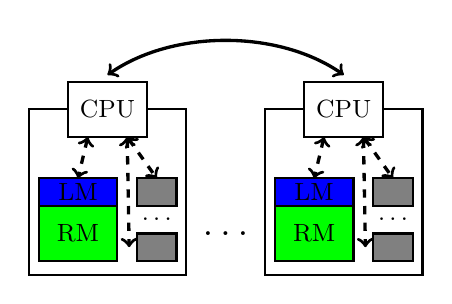
\begin{tikzpicture}[xscale=0.5, yscale=0.35]

	% \draw[thick, fill=white] (4, 14) rectangle (10, 19);
	% \draw (7, 18.25) node {{Coordinator}};
	% \draw[thick] (4.25, 14.5) rectangle (9.75, 17.5);
	% \draw (7, 17) node {\small{Partition$\to$Machine}};
	% \draw (4.25, 16.5) -- (9.75, 16.5);
	% \draw (7, 16) node {\small{Offset$\to$Partition}};
	% \draw (4.25, 15.5) -- (9.75, 15.5);
	% \draw (7, 15) node {\small{Key$\to$Offset} \footnotesize{(NoSQL only)}};
	%
	% \draw[very thick, dashed, gray, <->] (7, 13.75) -- (0, 12.5);
	% \draw[very thick, dashed, gray, <->] (7, 13.75) -- (5, 12.5);
	% \draw[very thick, dashed, gray, <->] (7, 13.75) -- (10, 12.5);
	% \draw[very thick, dashed, gray, <->] (7, 13.75) -- (15, 12.5);
	%
	\draw[very thick, black, <->] (-1, 12.25) to [out=45, in=135] (5, 12.25);
	% \draw[very thick, black, ->] (0.75, 13.25) -- (4, 12.25);
	% \draw[very thick, black, <-] (-1, 12.25) to [out=45, in=180] (0.5, 13.75);
	% \draw[very thick, black, ->] (0.5, 13.75) -- (9, 12.25);
	% \draw[very thick, black, <-] (-1, 12.25) to [out=45, in=180] (0.25, 14.25);
	% \draw[very thick, black, ->] (0.25, 14.25) -- (14, 12.25);

	% \draw[very thick, black, <->] (-0.5, 16.5) -- (-1.25, 12);
	% \draw (-0.5, 17.5) node {\small{\tt search(string str)}};

	\draw[thick, fill=white] (-3, 5) rectangle (1, 11); 
	\draw[thick, fill=white] (-2, 12) rectangle (0, 10); 
	\draw (-1, 11) node {\small{CPU}};
	% \draw (-1, 10.5) node {\small{Handler}};
	
	\draw[thick, fill=blue] (-2.75, 7.5) rectangle (-0.75, 8.5);
	\draw[thick, fill=green] (-2.75, 5.5) rectangle (-0.75, 7.5);
	\draw (-1.75, 8) node {\small{LM}};
%	\draw (-2.75, 7.5) -- (-0.75, 7.5);
	\draw (-1.75, 6.5) node {\small{RM}};
%	\draw (-2.75, 6.5) -- (-0.75, 6.5);
%	\draw (-1.75, 6) node {\small{K$\to$O}};

%	\draw[thick] (-0.25, 5.5) rectangle (0.75, 8.5);
	\draw[thick, fill=gray] (-0.25, 8.5) rectangle (0.75, 7.5);
	\draw[thick, fill=gray] (-0.25, 5.5) rectangle (0.75, 6.5);
	\draw (0.25, 7) node {\small{$\dots$}};

	\draw[very thick, black, dashed, <->] (-1.5, 10) -- (-1.75, 8.5);
	\draw[very thick, black, dashed, <->] (-0.5, 10) -- (0.25, 8.5);
	\draw[very thick, black, dashed, <->] (-0.5, 10) -- (-0.45, 6);

	\draw (2, 6.5) node {\Large{$\dots$}};

		\draw[thick, fill=white] (3, 5) rectangle (7, 11); 
		\draw[thick, fill=white] (4, 12) rectangle (6, 10); 
		\draw (5, 11) node {\small{CPU}};
		% \draw (5, 10.5) node {\small{Handler}};

		\draw[thick, fill=green] (3.25, 5.5) rectangle (5.25, 7.5);
		\draw[thick, fill=blue] (3.25, 7.5) rectangle (5.25, 8.5);
		\draw (4.25, 8) node {\small{LM}};
		\draw (4.25, 6.5) node {\small{RM}};

	%	\draw[thick] (-0.25, 5.5) rectangle (0.75, 8.5);
		\draw[thick, fill=gray] (5.75, 8.5) rectangle (6.75, 7.5);
		\draw[thick, fill=gray] (5.75, 5.5) rectangle (6.75, 6.5);
		\draw (6.25, 7) node {\small{$\dots$}};

		\draw[very thick, black, dashed, <->] (4.5, 10) -- (4.25, 8.5);
		\draw[very thick, black, dashed, <->] (5.5, 10) -- (6.25, 8.5);
		\draw[very thick, black, dashed, <->] (5.5, 10) -- (5.55, 6);

		% \draw[thick, black] (-3, 4.75) -- (-2.9, 4.5);
		% \draw[thick, black] (-2.9, 4.5) -- (1.75, 4.5);
		% \draw[thick, black] (1.75, 4.5) to [in=90, out=0] (2, 4.25);
		% \draw[thick, black] (2.25, 4.5) to [in=90, out=180] (2, 4.25);
		% \draw[thick, black] (2.25, 4.5) -- (6.9, 4.5);
		% \draw[thick, black] (7, 4.75) -- (6.9, 4.5);
		% \draw (2, 3.75) node {\tt SuccinctStore};


		% 	\draw[thick, fill=white] (8, 5) rectangle (12, 11);
		% 	\draw[thick, fill=white] (9, 12) rectangle (11, 10);
		% 	\draw (10, 11.5) node {\small{CPU}};
		% 	% \draw (10, 10.5) node {\small{Handler}};
		%
		% 	\draw[thick] (8.25, 5.5) rectangle (10.25, 8.5);
		% 	\draw (9.25, 8) node {\small{P$\to$M}};
		% 	\draw (8.25, 7.5) -- (10.25, 7.5);
		% 	\draw (9.25, 7) node {\small{O$\to$P}};
		% 	\draw (8.25, 6.5) -- (10.25, 6.5);
		% 	\draw (9.25, 6) node {\small{K$\to$O}};
		%
		% %	\draw[thick] (-0.25, 5.5) rectangle (0.75, 8.5);
		% 	\draw[thick, fill=gray] (10.75, 8.5) rectangle (11.75, 7.5);
		% 	\draw[thick, fill=gray] (10.75, 5.5) rectangle (11.75, 6.5);
		% 	\draw (11.25, 7) node {\small{$\dots$}};
		%
		% 	\draw[very thick, black, dashed, <->] (9.5, 10) -- (9.25, 8.5);
		% 	\draw[very thick, black, dashed, <->] (10.5, 10) -- (11.25, 8.5);
		% 	\draw[very thick, black, dashed, <->] (10.5, 10) -- (10.55, 6);


			% \draw[thick, black] (8, 4.75) -- (8.1, 4.5);
			% \draw[thick, black] (8.1, 4.5) -- (9.75, 4.5);
			% \draw[thick, black] (9.75, 4.5) to [in=90, out=0] (10, 4.25);
			% \draw[thick, black] (10.25, 4.5) to [in=90, out=180] (10, 4.25);
			% \draw[thick, black] (10.25, 4.5) -- (11.9, 4.5);
			% \draw[thick, black] (12, 4.75) -- (11.9, 4.5);
			% \draw (10, 3.75) node {\tt SuffixStore};


			% 	\draw[thick, fill=white] (13, 5) rectangle (17, 11);
			% 	\draw[thick, fill=white] (14, 12) rectangle (16, 10);
			% 	\draw (15, 11.5) node {\small{CPU}};
			% 	% \draw (15, 10.5) node {\small{Handler}};
			%
			% 	\draw[thick] (13.25, 5.5) rectangle (15.25, 8.5);
			% 	\draw (14.25, 8) node {\small{P$\to$M}};
			% 	\draw (13.25, 7.5) -- (15.25, 7.5);
			% 	\draw (14.25, 7) node {\small{O$\to$P}};
			% 	\draw (13.25, 6.5) -- (15.25, 6.5);
			% 	\draw (14.25, 6) node {\small{K$\to$O}};
			%
			% %	\draw[thick] (-0.25, 5.5) rectangle (0.75, 8.5);
			% 	\draw[thick, fill=gray] (15.75, 8.5) rectangle (16.75, 7.5);
			% 	\draw[thick, fill=gray] (15.75, 5.5) rectangle (16.75, 6.5);
			% 	\draw (16.25, 7) node {\small{$\dots$}};
			%
			% 	\draw[very thick, black, dashed, <->] (14.5, 10) -- (14.25, 8.5);
			% 	\draw[very thick, black, dashed, <->] (15.5, 10) -- (16.25, 8.5);
			% 	\draw[very thick, black, dashed, <->] (15.5, 10) -- (15.55, 6);

				% \draw[thick, black] (13, 4.75) -- (13.1, 4.5);
				% \draw[thick, black] (13.1, 4.5) -- (14.75, 4.5);
				% \draw[thick, black] (14.75, 4.5) to [in=90, out=0] (15, 4.25);
				% \draw[thick, black] (15.25, 4.5) to [in=90, out=180] (15, 4.25);
				% \draw[thick, black] (15.25, 4.5) -- (16.9, 4.5);
				% \draw[thick, black] (17, 4.75) -- (16.9, 4.5);
				% \draw (15, 3.75) node {\tt LogStore};


	\end{tikzpicture}
	}
%  	\end{minipage}
%  	\begin{minipage}[c]{0.19\textwidth}
% 	    \caption{\small{{\bf Methodology Overview:} We run real-world applications on a $5$-node Amazon EC2 cluster and emulate disaggregated architecture as follows. The memory accesses are captured into ``local cache'' accesses and ``remote memory'' accesses using an in-house implementation of a special instrumentation tool (SIT) described in \S\ref{sec:workloads}. The local disk accesses are captured using the {\tt blktrace} utility. Finally, all remote memory and disk accesses are captured using {\tt TCPdump}.}}
% 	\label{fig:system}
% %	\end{minipage}
% \end{figure}
% %
% %
% %
% \begin{figure}
%  \begin{minipage}{0.33\textwidth}
% 	\centering
	\hspace{0.1in}
	\subfigure[Understanding application requirements (\S\ref{sec:requirements})] {	
	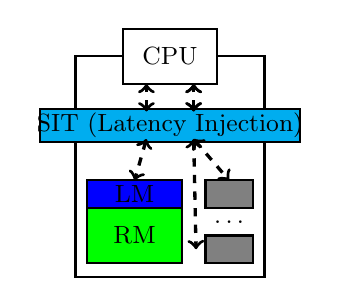
\begin{tikzpicture}[xscale=0.6, yscale=0.35]

	% \draw[thick, fill=white] (4, 14) rectangle (10, 19);
	% \draw (7, 18.25) node {{Coordinator}};
	% \draw[thick] (4.25, 14.5) rectangle (9.75, 17.5);
	% \draw (7, 17) node {\small{Partition$\to$Machine}};
	% \draw (4.25, 16.5) -- (9.75, 16.5);
	% \draw (7, 16) node {\small{Offset$\to$Partition}};
	% \draw (4.25, 15.5) -- (9.75, 15.5);
	% \draw (7, 15) node {\small{Key$\to$Offset} \footnotesize{(NoSQL only)}};
	%
	% \draw[very thick, dashed, gray, <->] (7, 13.75) -- (0, 12.5);
	% \draw[very thick, dashed, gray, <->] (7, 13.75) -- (5, 12.5);
	% \draw[very thick, dashed, gray, <->] (7, 13.75) -- (10, 12.5);
	% \draw[very thick, dashed, gray, <->] (7, 13.75) -- (15, 12.5);
	%
	% \draw[very thick, black, <->] (-1, 12.25) to [out=45, in=135] (5, 12.25);
	% \draw[very thick, black, ->] (0.75, 13.25) -- (4, 12.25);
	% \draw[very thick, black, <-] (-1, 12.25) to [out=45, in=180] (0.5, 13.75);
	% \draw[very thick, black, ->] (0.5, 13.75) -- (9, 12.25);
	% \draw[very thick, black, <-] (-1, 12.25) to [out=45, in=180] (0.25, 14.25);
	% \draw[very thick, black, ->] (0.25, 14.25) -- (14, 12.25);

	% \draw[very thick, black, <->] (-0.5, 16.5) -- (-1.25, 12);
	% \draw (-0.5, 17.5) node {\small{\tt search(string str)}};

	\draw[thick, fill=white] (-3, 5) rectangle (1, 13); 
	\draw[thick, fill=white] (-2, 14) rectangle (0, 12); 
	\draw (-1, 13) node {\small{CPU}};
	% \draw (-1, 10.5) node {\small{Handler}};
	
	\draw[thick, fill=cyan] (-3.75, 9.9) rectangle (1.75, 11.1); 
	\draw (-1, 10.5) node {\small{SIT (Latency Injection)}};
			
	\draw[thick, fill=blue] (-2.75, 7.5) rectangle (-0.75, 8.5);
	\draw[thick, fill=green] (-2.75, 5.5) rectangle (-0.75, 7.5);
	\draw (-1.75, 8) node {\small{LM}};
%	\draw (-2.75, 7.5) -- (-0.75, 7.5);
	\draw (-1.75, 6.5) node {\small{RM}};
%	\draw (-2.75, 6.5) -- (-0.75, 6.5);
%	\draw (-1.75, 6) node {\small{K$\to$O}};

%	\draw[thick] (-0.25, 5.5) rectangle (0.75, 8.5);
	\draw[thick, fill=gray] (-0.25, 8.5) rectangle (0.75, 7.5);
	\draw[thick, fill=gray] (-0.25, 5.5) rectangle (0.75, 6.5);
	\draw (0.25, 7) node {\small{$\dots$}};

	\draw[very thick, black, dashed, <->] (-1.5, 10) -- (-1.75, 8.5);
	\draw[very thick, black, dashed, <->] (-0.5, 10) -- (0.25, 8.5);
	\draw[very thick, black, dashed, <->] (-0.5, 10) -- (-0.45, 6);

	\draw[very thick, black, dashed, <->] (-1.5, 11) -- (-1.5, 12);
	\draw[very thick, black, dashed, <->] (-0.5, 11) -- (-0.5, 12);
	\draw[very thick, black, dashed, <->] (-0.5, 11) -- (-0.5, 12);

	\end{tikzpicture}
	}
%  	\end{minipage}\hfill
%  	\begin{minipage}[c]{0.19\textwidth}
% 	    \caption{\small{{\bf Methodology Overview:} We run real-world applications on a $5$-node Amazon EC2 cluster. To emulate end-to-end network latency, we inject artificial latencies for all ``remote memory'' and ``remote disk'' accesses and measure the impact of this latency to the application-level performance.}}
% 	\label{fig:system}
%	\end{minipage}
% \end{figure}
% %
% %
% \begin{figure}
%  \begin{minipage}{0.33\textwidth}
% 	\centering
	\hspace{0.1in}
	\subfigure[Exploring sufficiency of existing solutions (\S\ref{sec:existing})] {	
	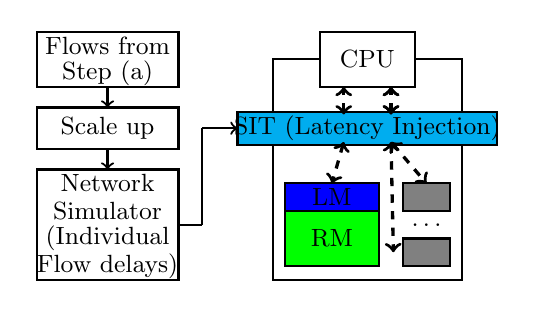
\begin{tikzpicture}[xscale=0.6, yscale=0.35]

	% \draw[thick, fill=white] (4, 14) rectangle (10, 19);
	% \draw (7, 18.25) node {{Coordinator}};
	% \draw[thick] (4.25, 14.5) rectangle (9.75, 17.5);
	% \draw (7, 17) node {\small{Partition$\to$Machine}};
	% \draw (4.25, 16.5) -- (9.75, 16.5);
	% \draw (7, 16) node {\small{Offset$\to$Partition}};
	% \draw (4.25, 15.5) -- (9.75, 15.5);
	% \draw (7, 15) node {\small{Key$\to$Offset} \footnotesize{(NoSQL only)}};
	%
	% \draw[very thick, dashed, gray, <->] (7, 13.75) -- (0, 12.5);
	% \draw[very thick, dashed, gray, <->] (7, 13.75) -- (5, 12.5);
	% \draw[very thick, dashed, gray, <->] (7, 13.75) -- (10, 12.5);
	% \draw[very thick, dashed, gray, <->] (7, 13.75) -- (15, 12.5);
	%
	% \draw[very thick, black, <->] (-1, 12.25) to [out=45, in=135] (5, 12.25);
	% \draw[very thick, black, ->] (0.75, 13.25) -- (4, 12.25);
	% \draw[very thick, black, <-] (-1, 12.25) to [out=45, in=180] (0.5, 13.75);
	% \draw[very thick, black, ->] (0.5, 13.75) -- (9, 12.25);
	% \draw[very thick, black, <-] (-1, 12.25) to [out=45, in=180] (0.25, 14.25);
	% \draw[very thick, black, ->] (0.25, 14.25) -- (14, 12.25);

	% \draw[very thick, black, <->] (-0.5, 16.5) -- (-1.25, 12);
	% \draw (-0.5, 17.5) node {\small{\tt search(string str)}};

	\draw[thick, fill=white] (-8, 5) rectangle (-5, 9); 
	\draw[thick, fill=white] (-8, 9.75) rectangle (-5, 11.25); 
	\draw[thick, fill=white] (-8, 12) rectangle (-5, 14); 
	\draw (-6.5, 8.5) node {\small{Network}};
	\draw (-6.5, 7.5) node {\small{Simulator}};
	\draw (-6.5, 6.5) node {\small{(Individual}};
	\draw (-6.5, 5.5) node {\small{Flow delays)}};
	\draw (-6.5, 10.5) node {\small{Scale up}};
	\draw (-6.5, 13.5) node {\small{Flows from}};
	\draw (-6.5, 12.5) node {\small{Step (a)}};
	\draw[thick, black, ->] (-6.5, 12) -- (-6.5, 11.25);
	\draw[thick, black, ->] (-6.5, 9.75) -- (-6.5, 9);
	\draw[thick, black, -] (-5, 7) -- (-4.5, 7);
	\draw[thick, black, -] (-4.5, 7) -- (-4.5, 10.5);
	\draw[thick, black, ->] (-4.5, 10.5) -- (-3.75, 10.5);

	\draw[thick, fill=white] (-3, 5) rectangle (1, 13); 
	\draw[thick, fill=white] (-2, 14) rectangle (0, 12); 
	\draw (-1, 13) node {\small{CPU}};
	% \draw (-1, 10.5) node {\small{Handler}};
	
	\draw[thick, fill=cyan] (-3.75, 9.9) rectangle (1.75, 11.1); 
	\draw (-1, 10.5) node {\small{SIT (Latency Injection)}};
			
	\draw[thick, fill=blue] (-2.75, 7.5) rectangle (-0.75, 8.5);
	\draw[thick, fill=green] (-2.75, 5.5) rectangle (-0.75, 7.5);
	\draw (-1.75, 8) node {\small{LM}};
%	\draw (-2.75, 7.5) -- (-0.75, 7.5);
	\draw (-1.75, 6.5) node {\small{RM}};
%	\draw (-2.75, 6.5) -- (-0.75, 6.5);
%	\draw (-1.75, 6) node {\small{K$\to$O}};

%	\draw[thick] (-0.25, 5.5) rectangle (0.75, 8.5);
	\draw[thick, fill=gray] (-0.25, 8.5) rectangle (0.75, 7.5);
	\draw[thick, fill=gray] (-0.25, 5.5) rectangle (0.75, 6.5);
	\draw (0.25, 7) node {\small{$\dots$}};

	\draw[very thick, black, dashed, <->] (-1.5, 10) -- (-1.75, 8.5);
	\draw[very thick, black, dashed, <->] (-0.5, 10) -- (0.25, 8.5);
	\draw[very thick, black, dashed, <->] (-0.5, 10) -- (-0.45, 6);

	\draw[very thick, black, dashed, <->] (-1.5, 11) -- (-1.5, 12);
	\draw[very thick, black, dashed, <->] (-0.5, 11) -- (-0.5, 12);
	\draw[very thick, black, dashed, <->] (-0.5, 11) -- (-0.5, 12);

	\end{tikzpicture}
	}
%  	\end{minipage}
%  	\begin{minipage}[c]{0.19\textwidth}
	    \caption{\small{(left) {\bf Workload Characterization:} We run real-world applications on a $5$-node Amazon EC2 cluster and emulate disaggregated architecture as follows. The memory accesses are captured into ``local cache'' accesses and ``remote memory'' accesses using an in-house implementation of a special instrumentation tool (SIT) described in \S\ref{sec:workloads}. The local disk accesses are captured using the {\tt blktrace} utility. Finally, all remote memory and disk accesses are captured using {\tt TCPdump}. (center) {\bf Understanding application requirements:} We run real-world applications on a $5$-node Amazon EC2 cluster. To emulate end-to-end network latency, we inject artificial latencies for all ``remote memory'' and ``remote disk'' accesses and measure the impact of this latency to the application-level performance. (right) {\bf Exploring sufficiency of existing solutions:} Same as Step 2, but the latencies injected for each flow are now a result of network simulation results. \rc{SIT representation imprecise}}}
	\label{fig:system}
%	\end{minipage}
\end{figure*}
%
\paragraphb{Memory and I/O blades}
Besides the local cache on CPU blades, disaggregating memory and storage is rather straightforward and has been an active research topic~\cite{x1, x2, x3}. We assume that each memory blade has a controller ASIC (or a lightweight processor) that implements address translation between the remote CPU's view of its address space and the addressing used internally within a blade{\footnote{\rqc{We should comment on metadata management here}}}. Furthermore, many I/O device controllers are beginning to support virtualization via the PCIe SR-IOV or MR-IOV features, which can be also leveraged in the disaggregated datacenter. We refer the reader to \cite{x1, x2, x3} for an in-depth discussion of hardware designs for disaggregated blades.

We assume that CPU blades access remote memory at the page granularity (4KB in x86) over the fabric. Typical memory access between CPU and DRAM in server-centric architecture occurs in the unit of cache-line size (64B in x86); however, we believe accessing memory at page granularity will be essential to better exploit spatial locality in common memory access patters and amortize the routing-trip latency more effectively. 
%\rqc{In addition, page-level access requires little or no modification to the virtual memory subsystems of hypervisor or operating system, and it is completely transparent to user-level applications. We further assume that those remotely accessed pages are not shared by multiple VMs at a given time, in order to not introduce cache coherence traffic across the network.

\paragraphb{Virtualization, resource allocation and scheduling}
The resource allocation and scheduling model in server-centric architecture is centered around virtual machines (VMs). In disaggregated datacenters, we do not need to restrict the resource allocation and scheduling model to VM-oriented architecture. We discuss how disaggregation enables new usage models in \S\ref{sec:discussion}. However, the VM model can still be useful to leverage the existing software infrastructure as well as running existing applications with little or no modification. As it is unclear how the resource allocation and scheduling will evolve in a disaggregated datacenter, we assume in this paper that resources are still utilized by aggregating them to form VMs, while each resource is now physically disaggregated across the datacenter.

The scheduler allocates resources by assigning resource blades (or a part of), configuring the resultant resource and address space assignments at the selected blades, and configuring the network that interconnects these blades. Depending of the scale of disaggregation, each rack may contain different types of resource blades and the scheduler may optimize for locality when it allocates resources to a job. The best layout of resource blades and the corresponding scheduler optimizations is a topic for future exploration.

\subsection{Design Knobs}
\label{ssec:assumptions}
The high-level architecture for disaggregated datacenters above leaves a number of design related questions open-ended, making only a set of essential assumptions based on feasibility and limitation of network fabric interconnecting the resource blades. Several of these design choices will have significant impact on the network fabric, the focus of this paper. We consider these choices as possible ``knobs'' in our study. We outline these knobs below, and analyze how these different knobs will impact the design and evolution of network fabric for disaggregated datacenters.

\begin{itemize}[leftmargin=*]
	\itemsep0em
	\item {\bf Local cache size:} how does the size of local cache affect the network fabric? Does increasing the cache size have a diminishing impact on network fabric?
	\item {\bf Scale of disaggregation:} whether disaggregation is performed at the rack-scale, pod-scale or the entire datacenter scale?
	\item {\bf Data placement:} whether or not locality in data placement and access essential for \dis?
	\item {\bf page size and access granularity:} ??
\end{itemize} 

% \paragraphb{VM as a computational unit}
% The current datacenter usage model is heavily based on the server-centric architecture. While physical servers in datacenters have evolved to server virtualization~\cite{cc} or other comparable technologies, they are still all centered around the concept of server, which aggregates slices to hardware resources within a server.
%
% In contrast, the usage model of a disaggregated datacenter does not necessarily follow the same approach; since computation, storage, and I/O functions can be completely disseminated across the datacenter, we do not need to restrict our usage model within the VM-oriented architecture. However, we note that the VM model can be still useful,
%
% \paragraphb{Local and remote memory}
% While disaggregation of I/O devices is relatively straightforward as discussed above, memory disaggregation brings a set of new challenges in terms of performance. Since memory access from CPUs must run at very high speed, similar to prior work, we assume that each CPU blade retains some amount of local memory that acts as a cache for remote memory; this disaggregating memory can be viewer as expanding the memory hierarchy to include a remote level.
%
% \paragraphb{Page-level remote memory access}
% We assume that CPU blades access remote memory at the page granularity (4KB in x86) over the fabric. While typical memory access between CPU and DRAM in traditional servers occurs in the unit of cache-line size (64B in x86), it is known that page level access better exploits spatial locality in common memory access patters and amortized the routing-trip latency more effectively. In addition, page-level access requires little or no modification to the virtual memory subsystems of hypervisor or operating system, and it is completely transparent to user-level applications. We further assume that those remotely accessed pages are not shared by multiple VMs at a given time, in order to not introduce cache coherence traffic across the network.
%
% \paragraphb{Block-level remote storage access}
% We assume that CPU blades access remote storage at the block granularity (4KB in x86) over the fabric. This is the storage access granularity between CPU and current storage devices (disk, SSD, etc) in traditional servers.

\subsection{Methodology Overview}
Figure~\ref{fig:system} gives a high-level overview of our methodology to explore the three questions outlined in \S\ref{sec:intro}. We provide details for each of the three steps in respective sections, but note that the requirements from the network fabric are heavily dependent on the underlying application. To that end, we explore a wide variety of applications varying from batch processing (long running background jobs), point queries (user facing short jobs) and stream processing (real-time data analytics), as outlined in Table~\ref{tab:workloads}. 
%Each of these applications typically have very different data read/write patterns, which will translate to very different traffic patterns in disaggregated datacenters. In fact, within these application types, each particular system and/or algorithm may have different patterns. To that end, we use all six different workloads across these three applications in our evaluation. These workloads are described in Table~\ref{tab:workloads}.

\begin{table*}
	\centering
	\caption{\small{Workloads and applications used in our evaluation. \rc{Describe data sizes for each application; and the datasets}}}
	\label{tab:workloads}
	\vspace{0.1in}
  \begin{tabular}{c|c|c|c}
	  \hline
		\textbf{Application} & \textbf{Application} & \textbf{System} & \textbf{Abbreviation}\\
		\textbf{domain} & \textbf{} & \textbf{} & \textbf{}\\\hline \hline
    Batch & WordCount & Spark and Hadoop & BC\\\hline
    Batch & TeraSort & Spark and Hadoop & BT\\\hline
    Batch & GraphEngine & GraphLab & BG\\\hline
    Point Queries & Key-value store & Memcached & PKV\\\hline
    Point Queries & Search & ElasticSearch & PS\\\hline
    Stream Processing & Wordcount & Storm & S\\\hline
    \hline
\end{tabular}
\end{table*}

%
% \subsection{Summary of key findings}
% \label{ssec:summary}
%
% \begin{itemize}
% 	\item Key Findings
% 	\begin{itemize}
% 		\item Network traffic
% 			\begin{itemize}
% 				\item no elephant/mice: implication?
% 				\item inter-arrival times no longer poisson: implication?
% 				\item traffic less bursty: implication?
% 				\item various design knobs for better control: implications?
% 			\end{itemize}
% 		\item Application Requirements
% 		\begin{itemize}
% 			\item 40Gbps suffices
% 			\item 5us RTT sufficient to maintain current performance
% 		\end{itemize}
% 		\item Existing Solutions enough?
% 	\end{itemize}
% \end{itemize}